\begin{frame}{From Page Image to Structured Output}
  \centering
  \resizebox{\textwidth}{!}{%
  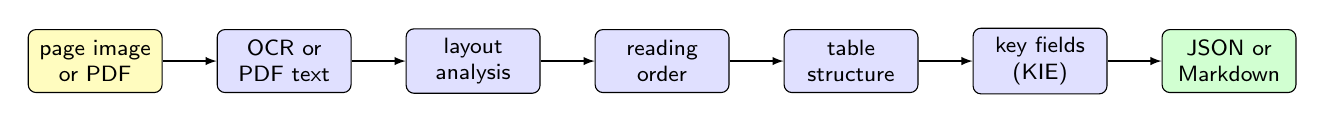
\begin{tikzpicture}[font=\sffamily\footnotesize, >=latex,
      stage/.style={draw, rounded corners=0.1cm, align=center, minimum width=1.7cm, minimum height=0.8cm, fill=blue!12},
      io/.style={stage, fill=yellow!25},
      res/.style={stage, fill=green!18}]
    \node[io]    (pg)  at (0,0)    {page image\\or PDF};
    \node[stage] (ocr) at (2.4,0)  {OCR or\\PDF text};
    \node[stage] (lay) at (4.8,0)  {layout\\analysis};
    \node[stage] (ro)  at (7.2,0)  {reading\\order};
    \node[stage] (tab) at (9.6,0)  {table\\structure};
    \node[stage] (kie) at (12.0,0) {key fields\\(KIE)};
    \node[res]   (out) at (14.4,0) {JSON or\\Markdown};
    \draw[->] (pg) -- (ocr);
    \draw[->] (ocr) -- (lay);
    \draw[->] (lay) -- (ro);
    \draw[->] (ro) -- (tab);
    \draw[->] (tab) -- (kie);
    \draw[->] (kie) -- (out);
  \end{tikzpicture}}\\[0.2em]
  {\scriptsize The modular pipeline: each stage is its own model and feeds the next.\par}
  \vspace{0.3em}
  {\scriptsize
  \begin{tabular}{>{\raggedright\arraybackslash}p{2.5cm} >{\raggedright\arraybackslash}p{4.6cm} >{\raggedright\arraybackslash}p{4.8cm}}
    \toprule
    \textbf{Sub-task} & \textbf{Output} & \textbf{Data point} \\
    \midrule
    OCR (optical character recognition) & words and their boxes, from pixels; born-digital PDFs already store both & FUNSD, end to end: Tesseract scores 3.4\%, Google Vision 76.4\% (edit-distance similarity) \\
    \addlinespace[0.15em]
    Layout analysis & labelled region boxes from object detection (covered in the CV course) & DocLayNet: 80{,}863 pages, 11 classes; best detector 76.8 mAP, annotators 82--83 \\
    \addlinespace[0.15em]
    Reading order & the order in which a person reads the regions & OCR's top-to-bottom order breaks columns; ReadingBank: 500{,}000 ordered pages \\
    \addlinespace[0.15em]
    Table structure recognition & rows, columns, header and spanning cells & TableFormer: grid from the table image, cell text from the PDF itself \\
    \addlinespace[0.15em]
    Key-information extraction (KIE) & values for named fields (e.g.\ vendor, date, total) or a form's question-answer pairs & FUNSD: 199 forms, about 10k linked entities: question, answer, header, other \\
    \bottomrule
  \end{tabular}\par}
  \vspace{0.2em}
  {\scriptsize Jaume et al., ``FUNSD,'' ICDAR-OST 2019, \href{https://arxiv.org/abs/1905.13538v2}{arXiv:1905.13538v2}, Tables I and IV; Pfitzmann et al., ``DocLayNet,'' KDD 2022, \href{https://arxiv.org/abs/2206.01062v1}{arXiv:2206.01062v1}, Table~2; Wang et al., ``LayoutReader,'' EMNLP 2021, \href{https://arxiv.org/abs/2108.11591v2}{arXiv:2108.11591v2}; Nassar et al., ``TableFormer,'' CVPR 2022.\par}
\end{frame}

\begin{frame}{Layout-Aware Encoders: LayoutLM and LayoutLMv3}
  \begin{columns}[T,onlytextwidth]
    \column{0.50\textwidth}
      \begin{itemize}\footnotesize\itemsep0.3em
        \item[\textcolor{red}{$\blacktriangleright$}] \textbf{LayoutLM:} BERT (covered earlier) plus a \textbf{2-D position embedding} of each OCR token's box, with corners scaled to a 0--1000 grid:
          \[ \mathbf{h}_i = \mathbf{e}_i + X(x_{0,i}) + Y(y_{0,i}) + X(x_{1,i}) + Y(y_{1,i}) \]
          {\scriptsize $\mathbf{h}_i$: transformer input for token $i$; $\mathbf{e}_i$: its usual BERT embedding; $(x_{0,i}, y_{0,i})$ and $(x_{1,i}, y_{1,i})$: top-left and bottom-right corners of its box; $X$, $Y$: learned lookup tables for $x$ and $y$.\par}
        \item[\textcolor{red}{$\blacktriangleright$}] \textbf{Pre-training:} mask tokens but keep their boxes, then predict the tokens, over 11M scanned pages whose words and boxes come from the Tesseract OCR engine. Downstream, Faster R-CNN (covered in the CV course) features of each token's image region are added.
        \item[\textcolor{red}{$\blacktriangleright$}] \textbf{LayoutLMv3:} no CNN; image patches enter through a linear layer, as in ViT (covered in the CV course). It masks 30\% of text tokens and about 40\% of patches, predicts both, and adds \textbf{word-patch alignment}: is the patch under an unmasked word masked?
      \end{itemize}
    \column{0.48\textwidth}
      \centering
      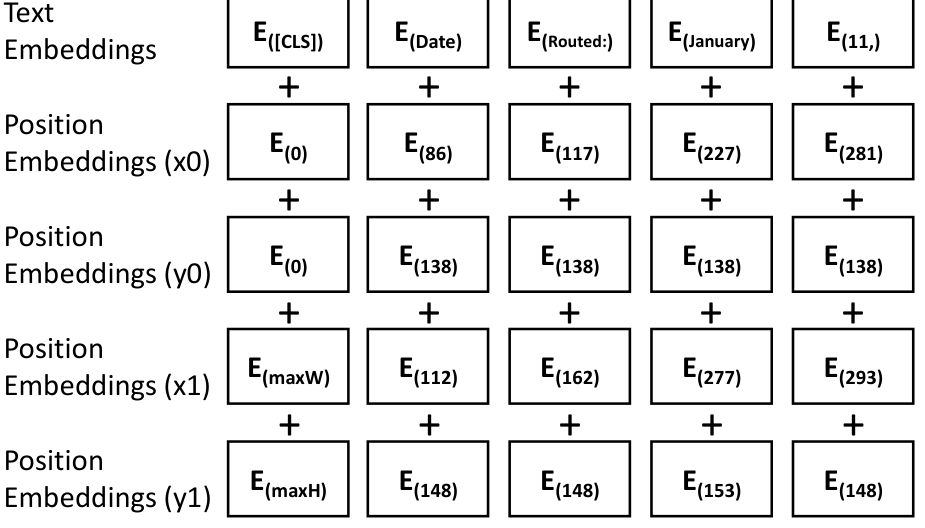
\includegraphics[width=0.9\linewidth,height=0.34\textheight,keepaspectratio]{images/nlp-security-enterprise/layoutlm_fig2_detail_position_embeddings.png}\\[0.2em]
      {\scriptsize Each token's text embedding plus four position embeddings of its box corners. Xu et al., ``LayoutLM: Pre-training of Text and Layout for Document Image Understanding,'' KDD 2020, \href{https://arxiv.org/abs/1912.13318v5}{arXiv:1912.13318v5}, Figure~2 (detail) and Table~1.\par}
      \vspace{0.3em}
      {\scriptsize
      \begin{tabular}{@{}p{2.4cm} p{2.3cm} p{0.8cm}@{}}
        \toprule
        \textbf{Model} & \textbf{Inputs} & \textbf{F1} \\
        \midrule
        BERT-base & text & 60.26 \\
        LayoutLM-base & + 2-D positions & 78.66 \\
        LayoutLM-base & + image regions & 79.27 \\
        LayoutLMv3-base & + image patches & 90.29 \\
        LayoutLMv3-large & + image patches & 92.08 \\
        \bottomrule
      \end{tabular}\par}
      {\scriptsize F1 for labelling FUNSD form entities. LayoutLMv3 uses one box per text segment, so it is not directly comparable. Huang et al., ``LayoutLMv3,'' ACM Multimedia 2022, \href{https://arxiv.org/abs/2204.08387v3}{arXiv:2204.08387v3}, Table~1.\par}
  \end{columns}
\end{frame}

\begin{frame}{Reading Without OCR: Donut}

  {\centering
  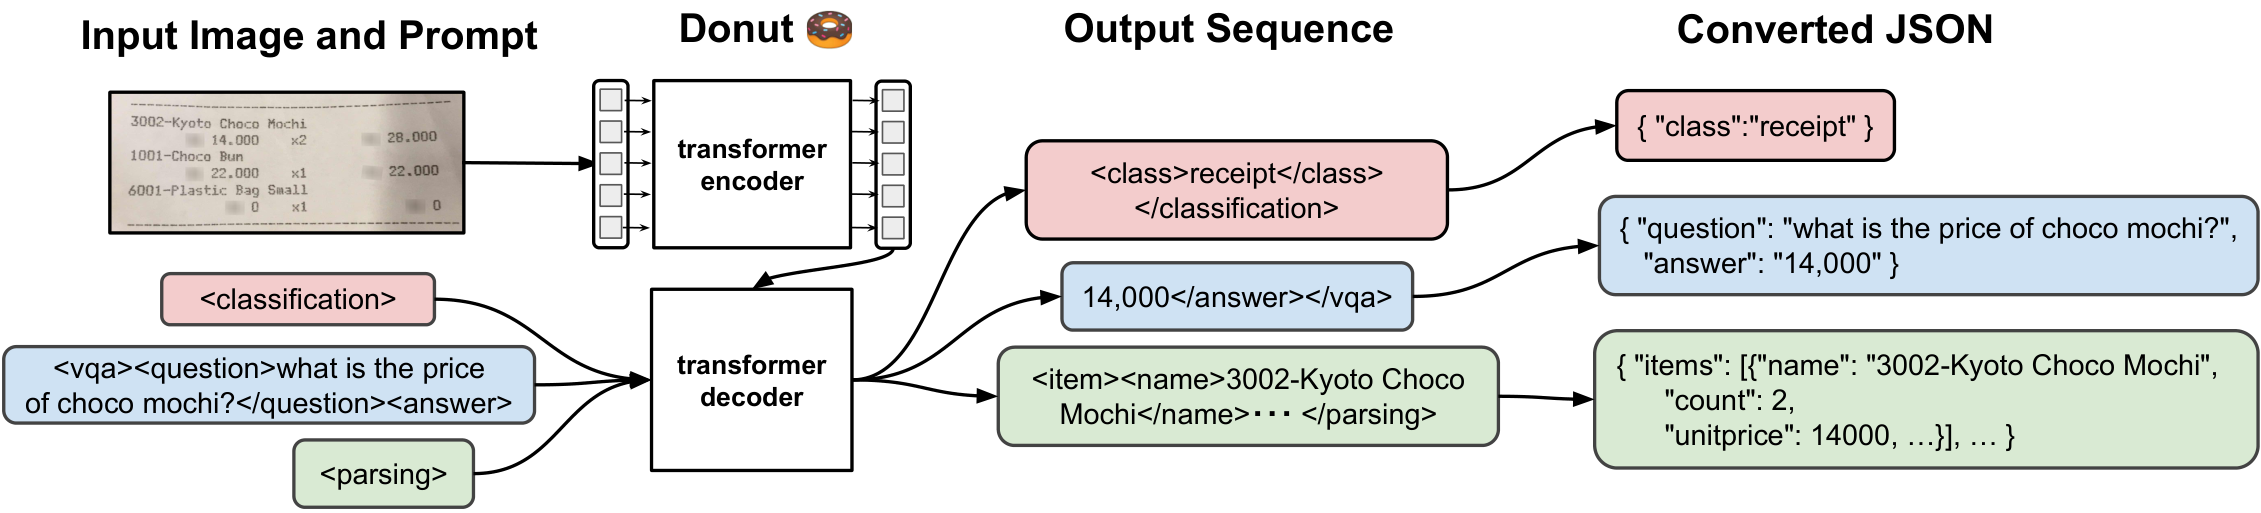
\includegraphics[width=\textwidth,height=0.33\textheight,keepaspectratio]{images/nlp-security-enterprise/donut_fig3_pipeline.png}\\[0.2em]
  {\scriptsize Kim et al., ``OCR-free Document Understanding Transformer,'' ECCV 2022, \href{https://arxiv.org/abs/2111.15664v5}{arXiv:2111.15664v5}, Figure~3; results: Tables 1--3 and Figure~6.\par}}
  \vspace{0.3em}
  \begin{columns}[T,onlytextwidth]
    \column{0.49\textwidth}
      \begin{itemize}\scriptsize\itemsep0.2em
        \item[\textcolor{red}{$\blacktriangleright$}] \textbf{OCR-free:} one network maps page pixels straight to the target text; no OCR engine, no word boxes.
        \item[\textcolor{red}{$\blacktriangleright$}] \textbf{Model:} a Swin Transformer encoder (covered in the CV course) reads a 2560$\times$1920 page; the decoder is the first four layers of BART, a pre-trained transformer encoder-decoder language model, emitting field tags that map one-to-one to JSON.
        \item[\textcolor{red}{$\blacktriangleright$}] \textbf{Pre-training is reading:} predict a page's text in reading order (``pseudo-OCR'') over 11M scanned pages and synthetic SynthDoG pages, 0.5M in each of four languages. A task prompt then selects classification, question answering or parsing.
      \end{itemize}
    \column{0.49\textwidth}
      \begin{itemize}\scriptsize\itemsep0.2em
        \item[\textcolor{red}{$\blacktriangleright$}] \textbf{Faster at equal accuracy:} RVL-CDIP document classification reaches 95.30\% at 752\,ms per page, against 95.25\% at 1{,}489\,ms for the OCR-based LayoutLMv2, OCR call included. On CORD receipts, field F1 is 84.1 against 78.9 for LayoutXLM, LayoutLMv2's multilingual version.
        \item[\textcolor{red}{$\blacktriangleright$}] \textbf{Weak spots:} DocVQA (covered earlier) scores 67.5 against 78.1 ANLS, a normalized edit-distance score; tiny text is lost at the fixed input resolution; one answer returned a different number from the same page.
        \item[\textcolor{red}{$\blacktriangleright$}] \textbf{Since then:} page-image retrieval (ColPali) and vision-language model (VLM) document parsers, both covered earlier, carry the OCR-free idea further.
      \end{itemize}
  \end{columns}
\end{frame}

\begin{frame}{Choosing a Parser and Feeding Retrieval}

  {\centering\scriptsize
  \begin{tabular}{>{\raggedright\arraybackslash}p{1.9cm} >{\raggedright\arraybackslash}p{4.9cm} >{\raggedright\arraybackslash}p{5.1cm}}
    \toprule
     & \textbf{Modular pipeline} (e.g.\ Docling) & \textbf{Generative parser} (Donut, VLMs) \\
    \midrule
    Text fidelity & copied from the PDF or OCR, ``without the risk of generating false content'' & generated token by token; on dense pages GPT-4o omitted, rewrote or completed content \\
    \addlinespace[0.15em]
    Tables, formulas & a model per element (TableFormer for tables); formulas need another & one model for every element; reading order learned end to end \\
    \addlinespace[0.15em]
    Speed, cost & 0.48\,s per page on an L4 GPU, 3.1\,s on 8 virtual x86 cores; OCR is the slowest step & olmOCR (7B, own GPUs): \$176 per million pages; GPT-4o batch API: \$6{,}240 \\
    \addlinespace[0.15em]
    Provenance & page and box for every item in lossless JSON; Markdown drops them & plain text (olmOCR) or JSON fields (Donut), without page coordinates \\
    \addlinespace[0.15em]
    On-premises & fully local, suited to sites with no network path to the outside & local only with open weights and GPUs; an API sends every page out \\
    \bottomrule
  \end{tabular}\par}
  \vspace{0.3em}
  \begin{itemize}\footnotesize\itemsep0.3em
    \item[\textcolor{red}{$\blacktriangleright$}] \textbf{Hybrid:} olmOCR's document-anchoring adds the PDF's own text blocks and coordinates to the VLM prompt; from the image alone, models tended to ``invent larger texts when the image data was ambiguous'' (see the hallucination section of this lecture).
    \item[\textcolor{red}{$\blacktriangleright$}] \textbf{For retrieval:} the parsed elements become the structure-aware chunks of the scalable RAG section. Keep each chunk's page and box, so every cited sentence opens as a highlighted region of its page.
  \end{itemize}
  \vspace{0.1em}
  {\scriptsize Livathinos et al., ``Docling,'' AAAI 2025 Workshop, \href{https://arxiv.org/abs/2501.17887v1}{arXiv:2501.17887v1}, Secs.~1--3, 5.4, 6; Poznanski et al., ``olmOCR,'' \href{https://arxiv.org/abs/2502.18443v3}{arXiv:2502.18443v3}, Sec.~2.2, App.~A, Table~6.\par}
\end{frame}
